
\chapter{间断有限元方法及 MLP 限制器的应用}
\label{chap:dg-mlp}

\section{间断有限元方法}
\label{sec:dg-method}

本文采用文献 \cite{Cockburn1998} 中介绍的间断有限元方法. 仍然考虑
守恒律方程
组 (\ref{eq:scaler-hyperbolic-conservation-law}). 单元 $T$ 上的有
限元空间取为局部 $k$ 阶多项式空间 $P^{k}(T)$. 间断有限元采用有限元
方法的框架, 但是采用 ``间断的'' 基函数, 即基函数的支集仅为当前单
元. 其有限元空间为,
\begin{equation}
  \label{eq:funciton-space-discontinuous-galerkin}
  V_{h} = \left\{ v_{h} \in L^{\infty}(\Omega) ; v_{h}|_{T} \in
    P^{k}(T), \forall T \in \mathcal{T} \right\}
\end{equation}
间断有限元方法就是在空间 $V_{h}$ 中寻找最佳近似解 ${{u}}_{h}$.
在 (\ref{eq:scaler-hyperbolic-conservation-law}) 式左右两侧乘任意
光滑函数 $v(x)$, 并在 $T_{j}$ 上积分, 得到其弱形式,
\begin{equation}
  \label{eq:scaler-hyperbolic-conservation-law-weak-form}
  \frac{\dd}{\dd t} \int_{T_{j}} u(x,t) ~ v (x) \dd x +
  \sum_{e\in \partial T_{j}} \int_{e} {\bf{f}} (u(x,t)) \cdot
  {\bf{n}}_{e,T_{j}} v(x) \dd \Gamma - \int_{T_{j}}
  {\bf{f}}(u(x,t)) \cdot \nabla v(x) \dd x =0,
\end{equation}
用数值积分处理后面两项积分项, 注意到两项分别为在单元边界的积分和在
单元内部的积分,
\begin{equation}
  \label{eq:DG-quadrature-rule}
  \begin{aligned}
    & \int_{e} {\bf{f}} (u(x,t)) \cdot {\bf{n}}_{e,T_{j}}
    v(x) \dd \Gamma \approx \sum_{l=1}^{L} \omega_{l} {\bf{f}}
    (u(x_{e,l},t)) \cdot {\bf{n}}_{e,T_{j}} v(x_{e,l}) \vert e
    \vert,\\
    & \int_{T_{j}} {\bf{f}}(u(x,t)) \cdot \nabla v(x) \dd x
    \approx \sum_{q=1}^{Q} \bar{\omega}_{q}
    {\bf{f}}(u(x_{T_{j},q},t)) \cdot \nabla v(x_{T_{j},q}) \vert T_{j} \vert.
  \end{aligned}
\end{equation}
其中 $x_{e,l}, x_{T_{j},q}$ 分别表示单元边界积分和单元内部积分的
积分点.

引入有限体积法中的数值通量 $h_{e,T_{j}}(x,t)$ 代替通量
项${\bf{f}}(u(x,t))\cdot {\bf{n}}_{e,T_{j}}$. 数值通量需要满足条
件 (\ref{eq:numerical-flux-condition}). 用近似解 $u_{h}$ 代替
$u$, 用 $v_{h}\in V(T_{j})$ 代替 $v$ 得到离散的弱形式,
\begin{equation}
  \label{eq:discrete-weak-form}
  \begin{split}
    \frac{\dd}{\dd t}& \int_{T_{j}} u_{h}(x,t) v_{h}(x) \dd x +
    \sum_{e\in\partial T_{j}} \sum_{l=1}^{L} \omega_{l} h_{e,T_{j}}
    \left( x_{e,l},t \right) v(x_{e,l}) \vert e \vert\\
    & - \sum_{q=1}^{Q} \bar{\omega}_{q} {\bf{f}}
    (u_{h}(x_{T_{j},q}, t)) \cdot \nabla v_{h} (x_{T_{j},q})
    \vert T_{j} \vert = 0, \quad \forall v_{h} \in V(T_{j}),
    \forall T_{j} \in \mathcal{T}.
  \end{split}
\end{equation}

记 $\left\{ \phi_{k} \right\}_{k=0}^{K}$ 为 $P^{k}(T)$ 的一组基,
在单元 $T_{j}$ 上有限元解可以按这组基分解为,
\begin{equation}
  \label{eq:decomposition-of-discontinuous-galerkin-solution}
  u_{h} |_{T_{j}} (x,t) = \sum_{k=0}^{K} u_{j}^{(k)} (t) \phi_{k} (x).
\end{equation}
记 ${\bf{U}}_{j}(t) = \left[ u_{j}^{(0)}, \cdots, u_{j}^{(K)}
\right]^{T}$ 为自由度向量. 引入单元 $T_{j}$ 上的单元质量矩阵,
\begin{equation}
  \label{eq:stiffness-matrix}
  M_{T_{j}} = \int_{T_{j}} {{\Phi}}_{T_{j}} (x)
  {{\Phi}}_{T_{j}}^{T} (x) \dd \Omega ,
  % \quad {{\Phi}}(x) = \left[
  %   \begin{array}{c}
  %     \phi_{0}\\
  %     \vdots\\
  %     \phi_{K}
  %   \end{array}
  % \right].
\end{equation}
其中 $\Phi_{T_{j}} = \left[ \phi_{0}, \cdots, \phi_{K}
\right]^{T}$ 为单元 $T_{j}$ 上的基函数向量.  $M_{T_{j}}$ 是一
个 $K \times K$ 的实对称矩阵. 在(\ref{eq:discrete-weak-form}) 中,
依次取测试函数 $v_{h}(x)$ 为所哟基函数 $\phi_{k}(x), k = 0,
\cdots, k$, 得到半离散形式的微分方程组,
\begin{equation}
  \label{eq:semi-discrecte-ode}
  \begin{split}
    M_{T_{j}} \left( \frac{\dd {\bf{U}}_{j}(t)}{\dd t} \right) &=
    - \sum_{e \in \partial T_{j}} \sum_{l=1}^{L} \omega_{l}
    h_{e,T_{j}} (x_{e,l},t) \vert e \vert \Phi_{T_{j}}
    (x_{e,l})\\
    & + \sum_{q=1}^{Q} \bar{\omega}_{q}
    {\bf{f}}(u_{h}|_{T_{j}},x_{T_{j},q}) \cdot \nabla
    \Phi_{T_{j}} (x_{T_{j},q}) \vert T_{j} \vert,
  \end{split}
\end{equation}

现假设有初值条件 $u(x, 0) = u_{0}(x)$, 采用标准的 $L^{2}$ 投影方
法将 $u_{0}$ 投影到有限元解空间 $V_{h}$, 可以得到初始离散解
$u_{h}(t=0) = \mathcal{P}_{V_{h}}(u_{0})$. $L^{2}$ 投影的等价形式
为,
\begin{equation}
  \label{eq:L2-projection}
  \int_{T_{j}} \left( u_{0} - u_{h}|_{T_{j}}(t=0) \right) \Phi_{T_{j}}
  \dd \Omega = 0.
\end{equation}
注意到 $u_{h}|_{T_{j}}(t=0) = {\bf{U}}_{j}^{T}(t=0) \cdot
\Phi_{T_{j}}$, 上式可以转化为,
\begin{equation}
  \label{eq:initial-degree-of-freedom}
  M_{T_{j}} {\bf{U}}_{j}(t=0) = \int_{T_{j}} u_{0} \Phi_{T_{j}}
  \dd \Omega
\end{equation}
(\ref{eq:initial-degree-of-freedom}) 式是关于单元 $T_{j}$ 上初始自
由度 ${\bf{U}}_{j}(t=0)$ 的线性方程组, 求解即可得单元上的初始
解 $u_{h}|_{T_{j}}(t=0)$.

% 基函数的选择?
当选择基函数 $\Phi_{T_{j}}$ 为一组正交基, 质量矩阵 $M_{T_{j}}$ 退
化为对角型, 这会给求解过程带来了很大的方便. 在下面的计算中, 采用文
献 \cite{Cockburn1998} 中的基函数, 相对应的三个自由度分别为三条边
的中点值. 容易验证这组基函数是相互正交的.
% 为了表述方便需要引入重心
% 坐标进行描述, 相关理论参考 ({\todo}附录 A)

\section{MLP 限制器的应用及数值算例}
\label{sec:mlp-apply}

高阶间断有限元方法同样会出现虚假数值震荡的问题. 将有限体积法中的限
制器概念引入到间断有限元方法中是解决该问题的一个有效的手段. 两者的
区别在于, 有限体积法限制的是重构所得到的函数, 而间断有限元方法解本
身就包含有高阶项. 例如, 二阶的间断有限元方法 $\mbox{DG}(P_{1})$的
解在每个单元上是线性函数, 因此可以自然的引
入(\ref{sec:MUSCL-on-unstru}) 节中介绍的有限体积法 MUSCL 类型斜率
限制器. 在保持单元平均值不变的前提下对数值解进行调整,
\begin{equation}
  \label{eq:MUSCL-DG}
  \tilde{u}_{h} (x,t) |_{T_{j}} = u_{j} + \alpha_{T_{j}}\left(
    u_{h}(x,t) |_{T_{j}} - u_{j} \right)
\end{equation}
在 (\ref{sec:improve-MLP-limiter}) 一节中我们分析了模板的选择对数
值格式的多维性质的影响. MLP 限制器由于使用了所有与当前单元共享顶点
的邻居单元作为限制器模板, 从而较好的解决了传统非结构网格方法描述高
维流体的多维性质方面的困难. 我们在非结构网格 $\mbox{DG}(P_{1})$ 计
算程序中实现了 (\ref{sec:improve-MLP-limiter}) 中对 MLP 限制器实施
策略的改进. 并与其 LCD 斜率限制器策略进行了对比.

\begin{description}
\item[线性波问题] 我们考虑线性波问
  题
  \begin{equation}
    \label{eq:linear-wave-problem-testcase}
    u_{t} + {\bf{a}} \cdot \nabla u = 0
  \end{equation}
  该算例常用于检验格式的正确性与数值精度. 当采用周期性边界条件,解
  析解图像在一定时间周期后会回到初始状态. 设定速度向
  量 ${\bf{a}}=(1,2)$为常量. 计算区域为 $[0,1] \times [0,1]$. 采用
  剖分矩形单元的方式生成 Scottish 类型的结构化非结构网
  格 \cite{Buffard2010}, 如图 (\ref{fig:structured-mesh-show}) 所
  示. 数值通量采用迎风通量. 时间推进采
  用 (\ref{sec:time-stepping-methods})一节中提到的二阶 SSP
  Runge-Kutta 方法. 边界条件采用周期性边界条件.
  \begin{figure}[htbp]
    \centering
    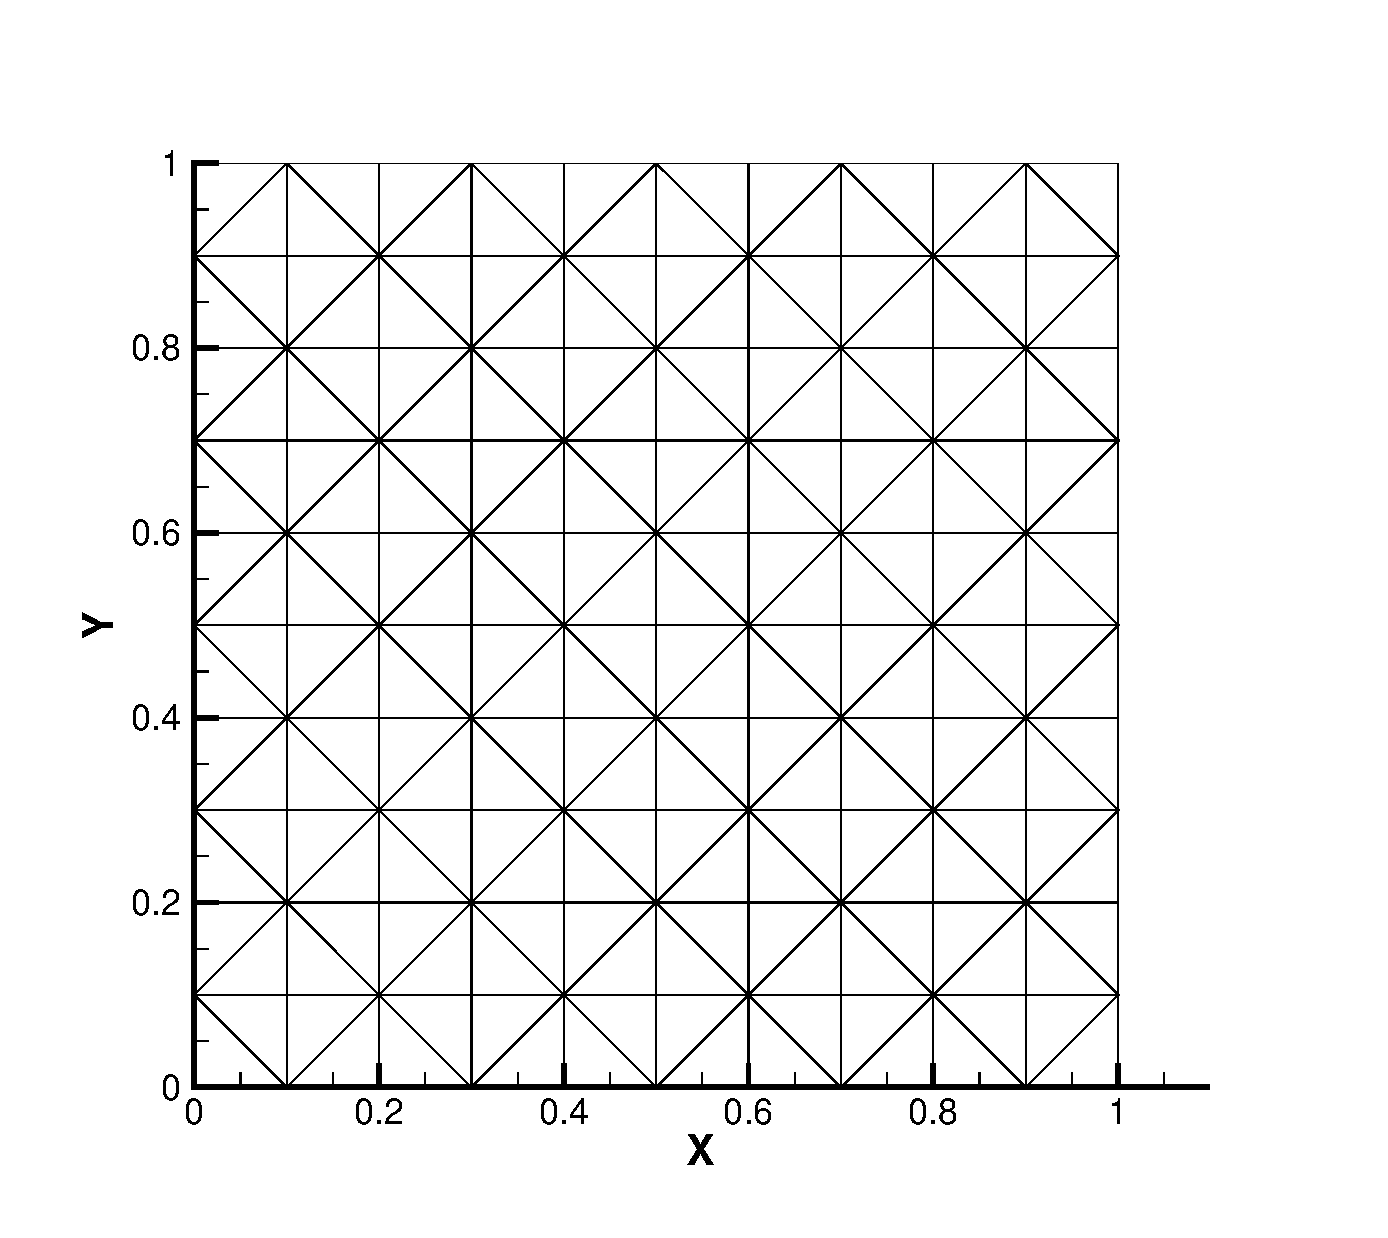
\includegraphics[height=2.0in]{./Pho/Chp3/mesh10X10.eps}
    \caption{测试所用网格}
    \label{fig:structured-mesh-show}
  \end{figure}
  我们考虑下面两种初值,
  \begin{itemize}
  \item Double Sine Wave 初值,
    \begin{equation}
      \label{eq:double-sine-wave}
      u_{0} = \sin(2\pi x) \sin (2\pi y), \quad (x,y) \in
      [0,1]\times [0,1],
    \end{equation}
    其精确解在时间 $t$ 为任意正整数时与初值重合. 在测试算例中对比
    了无限制器作用、LCD 限制以及 MLP 限制器三种情况. 并且采
    用$20\times 20 \times 2$、 $40\times 40 \times 2$、$80\times
    80 \times 2$ 以及 $160\times 160 \times 2$ 四套网格用于分析收
    敛阶.

    $L^{1}$ 误差以及收敛阶数等计算结果如
    表 (\ref{tb:accuracy-test}) 所示. 可以看到对于无限制器作用的情
    况 (第一组数据) $L^{1}$ 误差收敛阶数与理论相符, 保持二阶的收敛
    速度. LCD 限制器作用之后使得误差大幅增加, 收敛阶数甚至不到一
    阶, 说明限制器会引入很大的数值耗散. 而 MLP 限制器可以很好的保
    持收敛阶数, 甚至有高于二阶的收敛速率, 并且其误差与无限制器作用
    情形保持在同一个量级.
  \item 方形波初值,
    \begin{equation}
      \label{eq:square-wave-test-case}
      u_{0} = \left\{
        \begin{aligned}
          &1 &\quad & \mbox{if}~ 0.25 \le x,y \le 0.75\\
          &0 &\quad & \mbox{otherwise}
        \end{aligned}
      \right.
    \end{equation}
    该初值刻画了一个位于计算区域中间部分值为 $1$ 的高值区域, 其他
    区域值为 $0$. 而两部分的衔接处是间断. 该算例一方面用于测试算法
    是否能够有效的以高解析度的方式刻画间断, 另一方面也可以测试算法
    是否可以有效的抑制间断附近的虚假数值震荡. 在该算例的计算中, 采
    用 $80 \times 80 \times 2$ 的计算网格. 计算结果如
    图 (\ref{fig:square-wave-test-case}) 所示. 左侧的计算结果说明
    MLP 限制器可以较好的抑制数值震荡, 但是在间断附近会出现微小的
    震荡, 但是可以将其控制在允许的误差范围之内. 从两张图片的对比
    可以看出 MLP 限制器明显的减少了数值耗散, 从而提高了对间断的解
    析程度.
  \end{itemize}
\end{description}
\begin{center}
  \scriptsize
  \begin{table}
    \begin{tabular}{rrrr|rr|rr}
      % \hline
      &            & \multicolumn{2}{c}{No Limiter} &
      \multicolumn{2}{c}{LCD Limiter} & \multicolumn{2}{c}{MLP Limiter} \\
      \hline
      Grid  &  NElement  &    $L^{1}$ Error  &  Order  &  $L^{1}$ Error  &  Order  &   $L^{1}$ Error  &  Order  \\
      \hline
      20X20X2  &       800  &     9.0e-03  &      -  &      2.8e-01  &      -  &      2.0e-02  &      -  \\
      40X40X2  &      3200  &     2.0e-03  &    2.1  &      1.8e-01  &   0.63  &      3.5e-03  &    2.5  \\
      80X80X2  &     12800  &     4.9e-04  &    2.0  &      1.0e-01  &   0.79  &      6.7e-04  &    2.4  \\
      160X160X2  &     51200  &     1.2e-04  &    2.0  &      5.7e-02  &   0.89  &      1.4e-04  &    2.2  \\
      \hline
    \end{tabular}
    \caption{Double sine wave 算例, 精度测试. ($t=1.0$)}
    \label{tb:accuracy-test}
  \end{table}
\end{center}
\begin{figure}
  \begin{subfigure}{.5\textwidth}
    \centering
    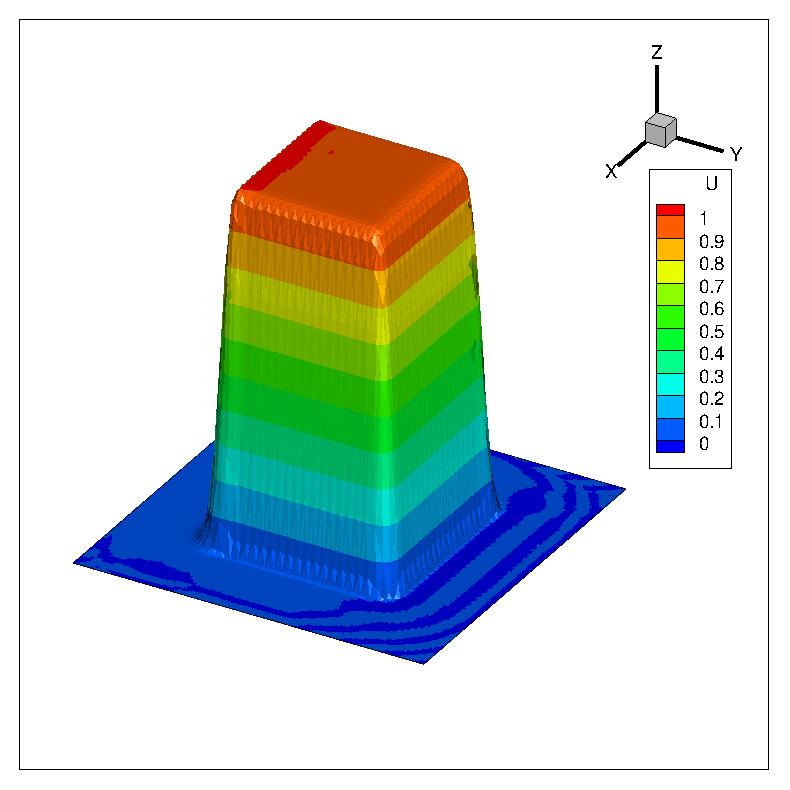
\includegraphics[width=.7\linewidth]{./Pho/Chp3/square_MLP_mesh80_3D.eps}
    \caption{MLP Limiter}
    \label{fig:sfig1}
  \end{subfigure}%
  \begin{subfigure}{.5\textwidth}
    \centering
    
\includegraphics[width=.7\linewidth]{./Pho/Chp3/square_Barth_mesh80_3D.eps}
    \caption{LCD Limiter}
    \label{fig:sfig2}
  \end{subfigure}
  \caption{Square Wave, $t=1.0$, $80\times 80 \times 2$ Grid.}
  \label{fig:square-wave-test-case}
\end{figure}

\begin{description}
\item[旋转对流问题(Solid-body rotation)] 描述的是按一致的角速度绕区域中心旋转的标量
  场 \cite{Leveque2004}. 首先考虑方
  程 (\ref{eq:linear-wave-problem-testcase}) 更一般的形式, 即速度
  矢量场非恒定的情形,
  \begin{equation}
    \label{eq:general-conservative-advection-equation}
    u_{t} + (u(x,y) u)_{x} + (v(x,y) u)_{y} = 0
  \end{equation}
  如果 $u(x,y), v(x,y)$ 满足下面这个式子,
  \begin{equation}
    \label{eq:divergence-free}
    u_{x}(x,y) + u_{y}(x,y) = 0,
  \end{equation}
  则速度场具有 divergence-free 性质, 即流场中穿过任意闭合曲面的净
  流量为零. 旋转对流问题的速度场就是满足这一特定的例子. 其定义为,
  \begin{equation}
    \label{eq:solid-body-rotation-velocity-field}
    u(x,y) = - (y - y_{0}), \quad v(x,y) = x - x_{0},
  \end{equation}
  描述了整个流场按逆时针方向绕中心点 $(x_{0},y_{0})$ 以恒定角速
  度 $\theta = 2\pi$ 旋转. 对于任意整数 $N$, 精确解在时间点 $t =
  2N\pi$ 与初始解重合.

  在数值实验中, 我们取计算区域为 $[0,1]\times[0,1]$. 采用 $100
  \times 100 \times 2$ 网格. 旋转中心点取为 $(x_{0},y_{0}) =
  (0.5,0.5)$. 初值包含一个偏离中心位置, 半径 $r_{0} = 0.15$ 的圆锥,
  \begin{equation}
    \label{eq:initial-condition-solid-body-rotation}
    u_{0}(x,y) =  \left\{
      \begin{aligned}
        & 1 - r(x,y) &\quad & \mbox{if}~ r(x,y) \le 1\\
        &0 &\quad & \mbox{otherwise}
      \end{aligned}
    \right.
  \end{equation}
  其中 $r(x,y) = \left( 1/r_{0} \right) \sqrt{(x-c_{x})^{2} + (y-
   c_{y})^{2}}$. $(c_{x},c_{y}) = (0.5,0.25)$ 为圆锥中心的坐标.
 计算终止时间为 $t_{end} = 2 \pi$. 条件数为 $C_{cfl} = 0.5$.

 计算结果如图 (\ref{fig:solid-body-rotation-test-case}) 所示. 其
 中左侧图像为 MLP 限制器的结果, 对比 LCD 限制器可以明显的降低数值
 耗散.

  % \begin{equation}
  %   \label{eq:solid-body-rotation-equation}
  %   u_{t} + {\bf{a}} \cdot \nabla u = 0, \quad {\bf{a}} = \left(
  %     -(y-0.5), (x-0.5) \right),
  % \end{equation}
\end{description}

\begin{figure}
  \begin{subfigure}{.5\textwidth}
    \centering
    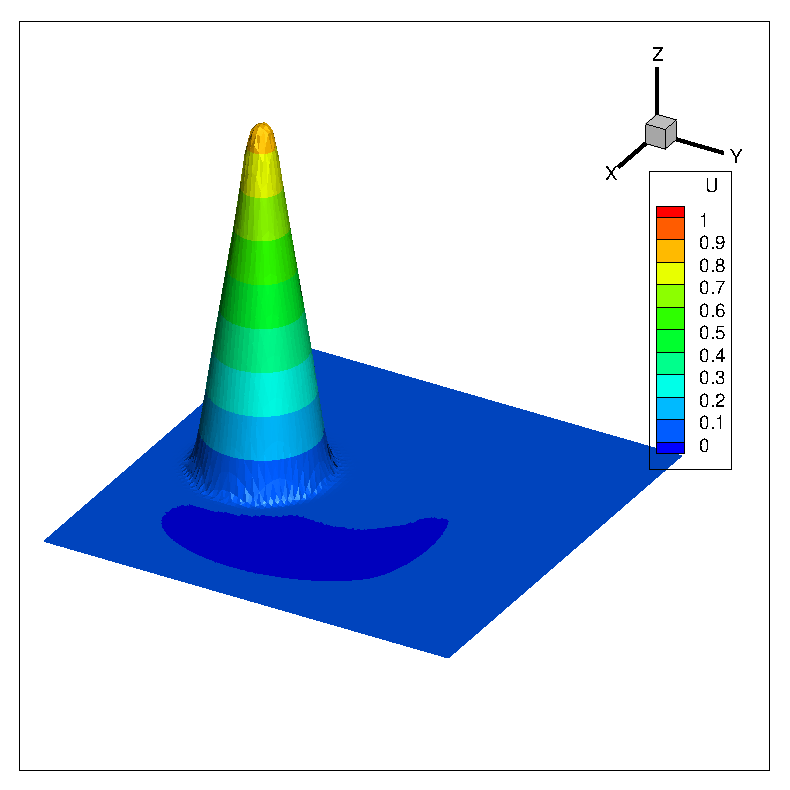
\includegraphics[width=.8\linewidth]{./Pho/Chp3/solidbodyrotation_MLP_mesh100.eps}
    \caption{MLP Limiter}
    \label{fig:sfig1}
  \end{subfigure}%
  \begin{subfigure}{.5\textwidth}
    \centering
    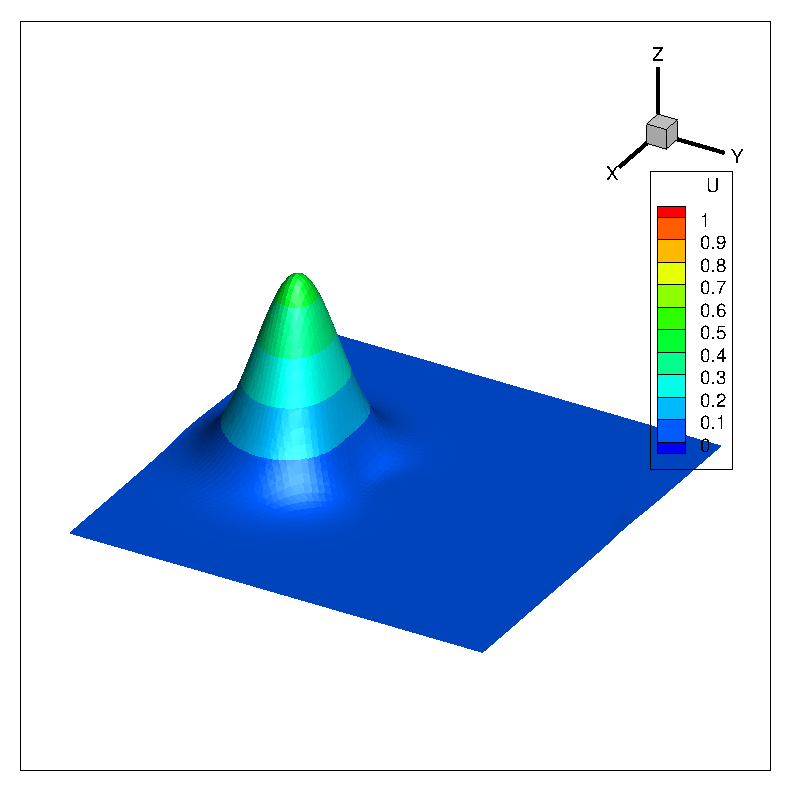
\includegraphics[width=.8\linewidth]{./Pho/Chp3/solidbodyrotation_Barth_mesh100.eps}
    \caption{LCD Limiter}
    \label{fig:sfig2}
  \end{subfigure}
  \caption{旋转对流问题, $t= 2 \pi$, $100\times 100 \times 2$ 网格.}
  \label{fig:solid-body-rotation-test-case}
\end{figure}
